\documentclass[tikz,border=10pt]{standalone}
\usetikzlibrary{patterns}
\usepackage{myfont}
\begin{document}
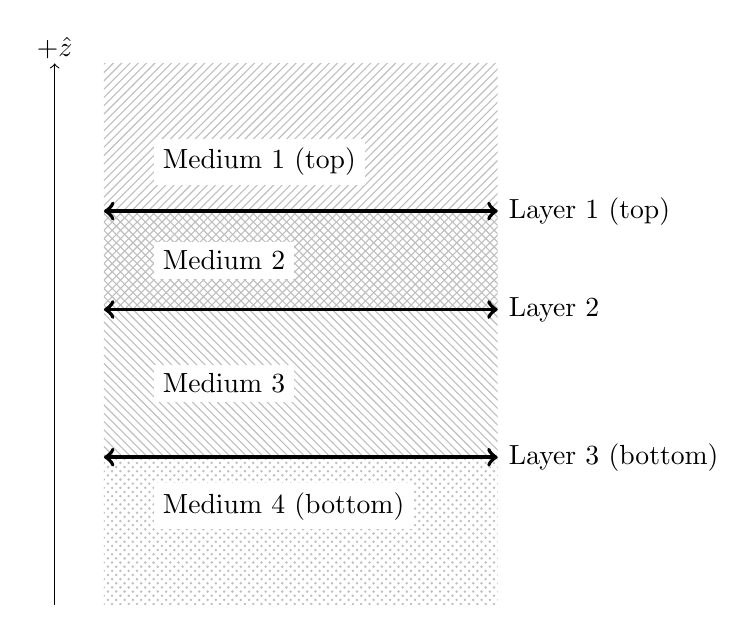
\begin{tikzpicture}[scale=1.25]
\coordinate (Layer0L) at (0, 0);
\coordinate (Layer0R) at (4, 0);
\coordinate (Layer1L) at (0, 1.5);
\coordinate (Layer1R) at (4, 1.5);
\coordinate (Layer2L) at (0, 2.5);
\coordinate (Layer2R) at (4, 2.5);
\coordinate (BottomL) at (0, -1.5);
\coordinate (BottomR) at (4, -1.5);
\coordinate (TopL) at (0, 4);
\coordinate (TopR) at (4, 4);
\coordinate (Z0) at (-0.5, -1.5);
\coordinate (Z1) at (-0.5, 4);
\fill[pattern=north east lines, pattern color=lightgray] (Layer2L) rectangle (TopR);
\fill[pattern=north west lines, pattern color=lightgray] (Layer0L) rectangle (Layer1R);
\fill[pattern=crosshatch, pattern color=lightgray] (Layer1L) rectangle (Layer2R);
\fill[pattern=crosshatch dots, pattern color=lightgray] (BottomL) rectangle (Layer0R);
    \draw[<->,line width=0.5mm] (Layer0L) -- (Layer0R) node [anchor=west] {Layer 3 (bottom)};
    \draw[<->,line width=0.5mm] (Layer1L) -- (Layer1R) node [anchor=west] {Layer 2};
    \draw[<->,line width=0.5mm] (Layer2L) -- (Layer2R) node [anchor=west] {Layer 1 (top)};
\draw[->] (Z0) -- (Z1) node [yshift=0.2cm] {$+\hat{z}$};
    \draw (0.5, 3) node [fill=white, anchor=west] {Medium 1 (top)};
    \draw (0.5, 2) node [fill=white, anchor=west] {Medium 2};
    \draw (0.5, 0.75) node [fill=white, anchor=west] {Medium 3};
    \draw (0.5, -0.5) node [fill=white, anchor=west] {Medium 4 (bottom)};
\end{tikzpicture}
\end{document}
